\subsubsection{The ABCD Method}

%A brief summary of this method follows below. 
%A detailed description can be found 
%in the supporting document~\cite{CMS_AN_2011-009}.

In this method the data are divided into four categories defined by boundaries on $\MET$ and the relative tracker 
isolation, $\ITRK/\ET$, of the electron candidate. The boundaries of the regions are chosen to minimize the overall 
statistical and systematic uncertainties on the signal yield.
Values of $\MET$ above and below the boundary of 25 GeV, together with $\ITRK/\ET$ values below 
the boundary of 0.04, define the regions A and B, respectively.
\begin{figure}[htbp]
\begin{center}
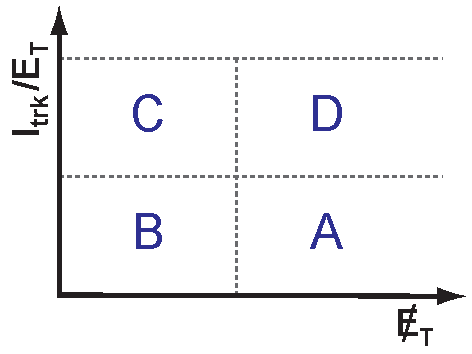
\includegraphics[width=0.35\textwidth]{figs/abcd.pdf}
\caption{The arrangement of the four categories of events used in the ABCD method. The vertical 
scale indicates increasing values of relative track isolation $\ITRK/\ET$
and the horizontal scale indicates increasing $\MET$.
%The dashed arrows show the directions of increasing signal purity.
}
\label{fig:abcde}
\end{center}
\end{figure}
Similarly, the regions above and below the $\MET$ boundary for $\ITRK/\ET$ values above 0.04, 
but below an upper $\ITRK/\ET$ bound of 0.2 (0.1) for electrons in the EB (EE), 
define the regions D and C, respectively. There is no upper bound for the $\MET$ values.
The different regions are shown graphically in Fig.~\ref{fig:abcde}, with region A 
having the greatest signal purity.
Combined regions are referred to as 'AB' (for A and B), for example.
The extracted signal corresponds to the entire ABCD region.

A system of equations is constructed relating the numbers of observed data events, $N_\mathrm{i}$, 
in each of the four regions ($\mathrm{i}$ = A, B, C and D) to the numbers 
of electroweak backgrounds, $E_\mathrm{i}$, QCD backgrounds, $Q_\mathrm{i}$, 
and signal events, $S_\mathrm{i}$. Several parameters should be determined from auxiliary 
measurements or simulations as shown in the following formulas: 

\begin{eqnarray}
 \label{eqABCD_Fa}
   f_\mathrm{A} & = & \frac{Q_\mathrm{A}}{Q_\mathrm{A} + Q_\mathrm{B}}  \\
  \label{eqABCD_Fb}
   f_\mathrm{D} & = & \frac{Q_\mathrm{D}}{Q_\mathrm{C} + Q_\mathrm{D}}  \\
  \label{eqABCD_EFFa}
   \epsilon_\mathrm{A} & = & \frac{S_\mathrm{A}}{S_\mathrm{A} + S_\mathrm{B}}  \\
  \label{eqABCD_EFFd}
   \epsilon_\mathrm{D} & = & \frac{S_\mathrm{D}}{S_\mathrm{C} + S_\mathrm{D}}  \\
  \label{eqABCD_EFFp}
   \epsilon_\mathrm{P} & = & \frac{S_\mathrm{A} + S_\mathrm{B}}{S_\mathrm{A} + S_\mathrm{B} + S_\mathrm{C} + S_\mathrm{D}} 
\end{eqnarray}

In this formulation, two parameters, $f_\mathrm{A}$ and $f_\mathrm{D}$, relate to the QCD 
backgrounds and are defined as the ratios of events with a fake electron candidate in the A and D 
regions to the number in the AB and CD regions, respectively. The two parameters represent the 
efficiency with which misidentified electrons pass the boundary on $\MET$ dividing
AD from BC. If the efficiency for passing the $\MET$ boundary is largely independent of the choice of
the boundaries on $\ITRK/\ET$, then these two parameters will be approximately equal. 
Assuming $f_\mathrm{A}=f_\mathrm{D}$ holds exactly 
leads to a simplification of the system of equations such that all direct dependence of the signal
extraction on parameters related to the QCD backgrounds is eliminated. For this idealized case there would be
no uncertainty on the extracted signal yield arising from modeling of QCD backgrounds. Detailed studies of the
data suggest this assumption holds to a good degree. A residual bias in the extracted signal arising from this
assumption is estimated directly from the data by studying a control sample 
obtained with inverted quality requirements on the electron candidate, 
and an appropriate small correction to the yield is applied (${\approx}0.37\%$).
A systematic uncertainty on the signal yield is derived from the uncertainty on this bias correction.
This contribution is small and is dominated by the uncertainty on signal
contamination in the control sample.

Three other important parameters relate to signal efficiencies: $\epsilon_\mathrm{A}$ 
and $\epsilon_\mathrm{D}$, which
are the efficiencies for signal events in the AB and CD regions, respectively, to pass the 
$\MET$ boundary, and $\epsilon_\mathrm{P}$, which is the efficiency for the electron candidate of a signal event 
to pass the boundary on relative track isolation dividing the AB region from the CD region under the 
condition that this electron already lies in the ABCD region. 
The first two of these, $\epsilon_\mathrm{A}$ and $\epsilon_\mathrm{D}$, are
estimated from models of the $\MET$ in signal events using the 
methods described in Section~\ref{sec:WsignalMETtemplate}.
The third parameter, $\epsilon_\mathrm{P}$, is measured from data using the \TNP method, described in
Section~\ref{sec:ELEefficiencies}, and is one of the dominant sources of 
uncertainty on the $\Wo$ boson yield before
considering the final acceptance corrections.

Electroweak background contributions are estimated from MC samples
with an overall normalization scaled through an iterative method with the signal yield. 
The electroweak contribution is subtracted from the observed data events in each of the four 
regions, $N_\mathrm{i} \rightarrow N_\mathrm{i} - E_\mathrm{i}$ ($\mathrm{i}$ = A, B, C and D).

Assuming that $f_\mathrm{A}$ = $f_\mathrm{B}$, the signal contained in the ABCD region, S, can 
be obtained from the following formula:

\begin{eqnarray}
 \label{eqABCD_S}
   \alpha S^2 + b S + c & = & 0 
\end{eqnarray}

with coefficients, 

\begin{eqnarray}
 \label{eqABCD_Sa}
   \alpha & = & \epsilon_\mathrm{P}(\epsilon_\mathrm{P} - 1)(\epsilon_\mathrm{A} - \epsilon_\mathrm{D})   \\
  \label{eqABCD_Sb}
   b & = & N_\mathrm{A}(1 - \epsilon_\mathrm{D})(1 - \epsilon_\mathrm{P}) - N_\mathrm{B}\epsilon_\mathrm{D}(1 - \epsilon_\mathrm{P}) + N_\mathrm{C}\epsilon_\mathrm{A}\epsilon_\mathrm{P} - N_\mathrm{D}\epsilon_\mathrm{P}(1 - \epsilon_\mathrm{A})  \\
  \label{eqABCD_Sc}
   c & = & N_\mathrm{B}N_\mathrm{D} - N_\mathrm{A}N_\mathrm{C}
\end{eqnarray}

The extracted yield with respect to the choice of boundaries in relative track isolation and $\MET$ is 
sensitive to biases in $\epsilon_\mathrm{P}$ and the QCD electron misidentification rate 
bias correction described above, respectively. 
The yield is very stable with respect to small changes in these selections, 
giving confidence that these 
important sources of systematic uncertainty are small.

The following signal yields are obtained:
$136\,003 \pm 498\,\mathrm{(stat.)}$ for the inclusive sample, $81\,525 \pm 385\,\mathrm{(stat.)}$ 
for the $\Wpen$ sample, and $54\,356 \pm 315\,\mathrm{(stat.)}$ for the $\Wmen$ sample.
%with negligible correlation between the $\Wp$ and $\Wm$ yields.
The ratios of the inclusive, $\Wpen$, and $\Wmen$ yields between this method and the parameterized
QCD shape are $0.998 \pm 0.007$, $0.999 \pm 0.007$, and $0.993 \pm 0.007$, respectively, considering
only the uncorrelated systematic uncertainties between the two methods.

